\documentclass[onecolumn, draftclsnofoot,10pt, compsoc]{IEEEtran}
\usepackage{graphicx}
\usepackage{url}
\usepackage{setspace}
\usepackage{cite}
\graphicspath{{./images/}}

\usepackage{geometry}
\geometry{textheight=9.5in, textwidth=7in}

% 1. Fill in these details
\def \CapstoneTeamName{		The Cleverly Named Team}
\def \CapstoneTeamNumber{		58}
\def \GroupMemberOne{			Daniel Grocki}
\def \GroupMemberTwo{			Austin Sanders}
\def \GroupMemberThree{			Owen Loughran}
\def \GroupMemberFour{			David Jansen}
\def \GroupMemberFive{			Brendan Byers}
\def \CapstoneProjectName{		Software product life cycle transformation with Docker container technology}
\def \CapstoneSponsorCompany{	HP}
\def \CapstoneSponsorPerson{		Bryan Crampton}

% 2. Uncomment the appropriate line below so that the document type works
\def \DocType{		%Problem Statement
				Requirements Document
				%Technology Review
				%Design Document
				%Progress Report
				}
			
\newcommand{\NameSigPair}[1]{\par
\makebox[2.75in][r]{#1} \hfil 	\makebox[3.25in]{\makebox[2.25in]{\hrulefill} \hfill		\makebox[.75in]{\hrulefill}}
\par\vspace{-12pt} \textit{\tiny\noindent
\makebox[2.75in]{} \hfil		\makebox[3.25in]{\makebox[2.25in][r]{Signature} \hfill	\makebox[.75in][r]{Date}}}}
% 3. If the document is not to be signed, uncomment the RENEWcommand below
\renewcommand{\NameSigPair}[1]{#1}

%%%%%%%%%%%%%%%%%%%%%%%%%%%%%%%%%%%%%%%
\begin{document}
\begin{titlepage}
    \pagenumbering{gobble}
    \begin{singlespace}
        \hfill 
        % 4. If you have a logo, use this includegraphics command to put it on the coversheet.
        %\includegraphics[height=4cm]{CompanyLogo}   
        \par\vspace{.2in}
        \centering
        \scshape{
            \huge CS Capstone \DocType \par
            {\large\today}\par
            \vspace{.5in}
            \textbf{\Huge\CapstoneProjectName}\par
            \vfill
            {\large Prepared for}\par
            \Huge \CapstoneSponsorCompany\par
            \vspace{5pt}
            {\Large\NameSigPair{\CapstoneSponsorPerson}\par}
            {\large Prepared by }\par
            Group\CapstoneTeamNumber\par
            % 5. comment out the line below this one if you do not wish to name your team
            %\CapstoneTeamName\par 
            \vspace{5pt}
            {\Large
                \NameSigPair{\GroupMemberOne}\par
                \NameSigPair{\GroupMemberTwo}\par
                \NameSigPair{\GroupMemberThree}\par
                \NameSigPair{\GroupMemberFour}\par
                \NameSigPair{\GroupMemberFive}\par
            }
            \vspace{20pt}
        }
        \begin{abstract}
        % 6. Fill in your abstract    
            	This document will detail the requirements of the container management system we are working on for HP’s PageWide Web Press printers. It will outline the purpose and scope of our project, as well as the specific limitations, definitions, and performance metrics for us to follow as we prepare to implement our ideas. Beyond this the document will define the functionality our project should provide, and the resultant usefulness that HP desire.

        \end{abstract}     
    \end{singlespace}
\end{titlepage}
\newpage
\pagenumbering{arabic}
% 7. uncomment this (if applicable). Consider adding a page break.
%\listoffigures
%\listoftables
\clearpage

% 8. now you write!


\section{Introduction}

\subsection{Purpose}

The purpose of this Requirements Document is to define the expectations of the "Software product life cycle transformation with Docker container technology" project. This document will lay out our plans for this project and provide clear specifications for us to follow. It also provides a clear agreement between us and the client about what is required for this project. 

\subsection{Scope}

The purpose of this project is to create a container management system for HP’s PageWide Web Press printers. The software we create will be a prototype of the system that HP wants to implement on their system. The goal is to containerize services to utilize less resources on the servers, as well as improve scaling. We will use Docker to containerize the services and Kubernetes to manage these containers. Our team will start by focusing on Hp’s Linux based servers. If our implementation on the Linux servers are successful we will move on to containerizing their Windows servers.
	
\subsection{Definitions}
\begin{itemize}
    \item \textbf{Docker:} Open source software platform to create, deploy and manage virtualized application containers on a common operating system\cite{tech}.
    
\item \textbf{Kubernetes:} Open source system used to manage Linux containers across private, public and hybrid cloud environments\cite{tech}.

\item \textbf{Application Containerization:} OS-level virtualization method used to deploy and run distributed applications without launching an entire virtual machine\cite{tech}.

\item \textbf{Docker Image:} A file, comprised of multiple layers, used to execute code in a Docker container\cite{tech}.

\item \textbf{Kubernetes Pod:} Smallest deployable computing units in the open source Kubernetes container scheduling and orchestration environment\cite{tech}.

\item \textbf{Server Operating System:} an operating system specifically designed to run on servers, which are specialized computers that operate within a client/server architecture to serve the requests of client computers on the network\cite{tech}.

\item \textbf{Linux Server:} Linux-based server operating system\cite{tech}.

\item \textbf{Windows Server:} Windows-based server operating system\cite{tech}.

\end{itemize}	

\section{Overview}
For this project we will be using both Docker and Kubernetes in order to create our containers for the HP PageWide Web Press. Docker is a very popular containerization software, containers are used to package code along with all of it’s necessary dependencies. This allows for code to reliably and more easily be ran on different environments. Within Docker a container begins as an image which holds the necessary code, runtime, system code, system libraries and the settings. These images become containers at run time\cite{kub}. 

Kubernetes is an open source software developed by Google that will be used as a way to manage the containers. Kubernetes will provide us with way to automate the deployment of our containers, scale them properly, and manage the applications that are developed using our containers. Each part of a process will become containerized, what Kubernetes does is throw all of these containers in to something referred to as a pod. This pod is pretty much a container that holds a group of containers which allows us to properly manage our entire process\cite{docker}. 

Our primary goal is to containerize the HP PageWide WordPress process on HP’s server stacks. Currently HP has two separate server types, Linux and Windows, that we will be containerizing their different services on. Our primary focus is on the Linux servers because there are more of them and they contain more of the services. As a group we need to figure out how to containerize both HP’s own services and the external services that they use. Once we have these services in containers we need to work on getting the containers to properly communicate with each other. After the containers are correctly communicating with each other we will use Kubernetes to throw the containers in to a pod and use it to manage the entire process.

Benefits of containing the entire printing process for HP include portability between their different environments, scaling on their server stacks, and no down time for updates. Currently HP can only run a single process on each server stack. This is because if they attempted to do multiple they would have issues keeping the two processes from interfering with one another. One of our goals is to allow two processes to run on a single server stack, with the use of Docker and Kubernetes this should be possible. HP will also be capable of updating their services individually when they are containerized. Rather than having to take down the entire process each container can be updated on their own. This means that there will be no downtime for the entire process because Docker allows you to create a new updated image and swap it out with the current image almost instantaneously. If our group is successful in our implementation on the Linux servers we will move on to begin the implementation on their Windows servers.

 





\section{Specific Requirements}

During development, code should be able to be checked into a source control system. Docker images for testing must be able to be created from this source code that can locally or a test stack. Once source code is ready, it will be commited to the version control tool Git. There will be a public GitHub repository to hold the information. 

There will be a continuous integration tool, Jenkins, that will run unit tests on the code and build Docker images. Once these images are successfully built, they can be pushed to Dockerhub. 

The code being written will model the services that HP actually uses for their printing. It will be written in Groovy with Gradle being used to help with dependencies. These models will then be used for testing the system.

Once a collection of images has been marked for a software release, they must be testable. The entire system must be easily buildable and upgradable for ease of testing. The system should allow for brand new images to be added as well as update existing images. It is also critical that the services inside of the containers can have their health monitored. The services that are containerized have health checks to determine their state and to see if they are working effectively. The containers must allow a way to access that information either through Kubernetes looking at the container, or the service inside reporting that information to the system. 

	Once the software has been successfully tested, there must be a deployment system for customers. It is required that there is a way to deploy the software release with the updated images to customers. This must be able to be done in two ways. For customers that are connected to the cloud, a remote deploy should be available to them. The system should be able to deploy the software release over the internet/cloud and be able to update all the customer systems that are connected. The second way we need to be able to deploy a software release is locally. For customers that are not connected to the cloud, there must be a way to manually deploy the new release locally on site. 
	
	In addition, when a new software release is deployed, Kubernetes must implement the rollback feature. If there is an issue, either on a local or remote deploy, the system should rollback to the previous working release and resume without interruption. Remote monitoring of the services is also required here. The status of the services running in the containers should be know and should be able to be monitored by the system. 


\subsection{User Characteristics}

There are 3 major groups that will be using this system, they are R\&D, System Test, and DevOps. As this technology is still rather new to HP, there is a chance then these groups will not have worked with Kubernetes or Docker before.

\subsection{External interfaces}

This system should allow Development, System Test, and DevOps to interface with the system. Development should be able to produce images and test them in a test environment. Their finished images should get build with a continuous integration tool such as Jenkins. 

System Test should be able to install a collection of images to the system. The system should also be able to output some statistics and data about the services running in the containers for System Test engineers to analyze. 

DevOps should be able to deploy the release to the customers over cloud or over a local method. The system should output health metrics for DevOps engineers to look at. 

\subsection{Functions}

The system will take multiple things as input. The primary input will be new updates to services. Since there are monthly updates, the system will be frequently receiving new images. When it receives a new image, the image should already have been built and successfully ran during the build process. When it receives this image it should then store it in it’s database. When we are ready to push the new image to the client systems, we should be able to push the one that we added to the database. This should eventually output a new update to the containers that are running the services. If there is any errors in the deployment of the updated container, Kubernetes should roll back to the previous working version.



\subsection{Usability Requirements}

One objective for this system is for it to decrease the amount of hardware that we need to use. Since this system will be used on actual hardware, making the services more efficient will in turn decrease the resources needed on each physical box. With the services needing less resources, we can run more services on a single box which should increase efficiency and decrease the amount of actual hardware that is needed. 

There are also usability requirements for the rolling update feature of the system. The rolling update should be effective in the sense that they successfully update the images on the client system. These images should be updated without causing the client system to stall or restart. Once the images are updated, new containers should be deployed from these images. If there is an issue with these new containers, the system should revert back to the old images. This should increase the efficiency of the entire container update process for the clients. 

\subsection{Performance Requirements}

The actual numbers for performance have yet to be decided, but the key feature is that a set of services should take up less resources on a server. This means that they should take up less RAM, CPU, and possibly even Memory. In addition the containerized services must run at least as fast as they did before they were containerized if not faster. Kubernetes must be able to network the containers together in a way that ensures the same level of efficiency as there was before they were containerized. 


\subsection{Limitations}

One source of limitations for this system is what HP servers can support. Since we will be deploying these containerized services to HP’s servers, we must make sure that the servers can support the number of containers we want to spin up on them. Depending on the size of the containers and any overhead required for their management, we may not be able to put as many containers on a server as we may need or want. 

Another source of limitations involves the the rolling updates we plan to implement with Kubernetes. Typically, Kubernetes and Docker make use of cloud services for these rolling updates. With everything living in the cloud, it makes it very simple to push a new update out to all the systems and allow for rollback if there is an error. Kubernetes is designed with this cloud infrastructure in mind and we don’t know how difficult it will be to take advantage of these features if not all of our systems can make use of the cloud. Most of the customer systems that this new container management system would affect not have an issue with a cloud based system. However, some of HP’s customers that would use this can’t support a cloud infrastructure. The features that we can implement with Kubernetes such as this rolling release may be limited by this fact. We will have to determine if we can make use of these Kubernetes features in both a cloud based environment and an older non cloud based environment. 

\subsection{Timeframe}

This gant chart outlines the timeframe we have in mind for completing each aspect of our project.
\begin{center}
    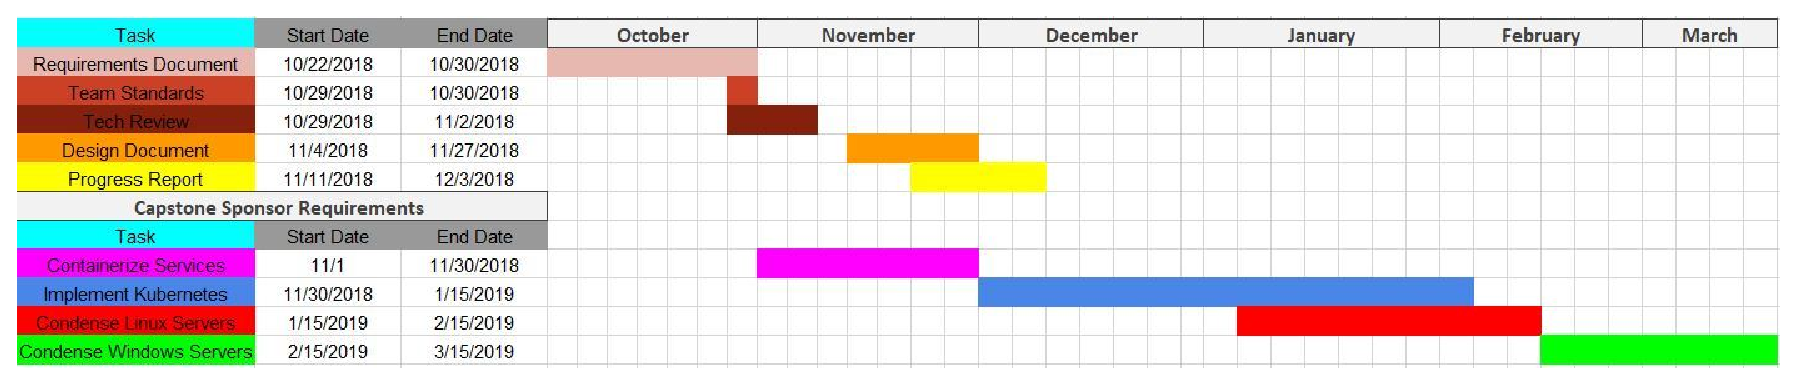
\includegraphics[width=\textwidth, height=5cm]{gant.eps}
\end{center}



\bibliographystyle{ieeetr}
\bibliography{references}

\end{document}
